\subsection{Sciency, technical stuff}

\begin{frame}{Things we do in \ab{} calculations}
    \begin{itemize}
        \item Electronic structure computation
        \item Optimize input crystal/molecular structures
        \item Phonon vibrational spectra computation
        \item Helmholtz free energy calculation at finite temperature
        \item Linear elastic constants
        \item More...
    \end{itemize}
    \begin{figure}[H]
        \centering
        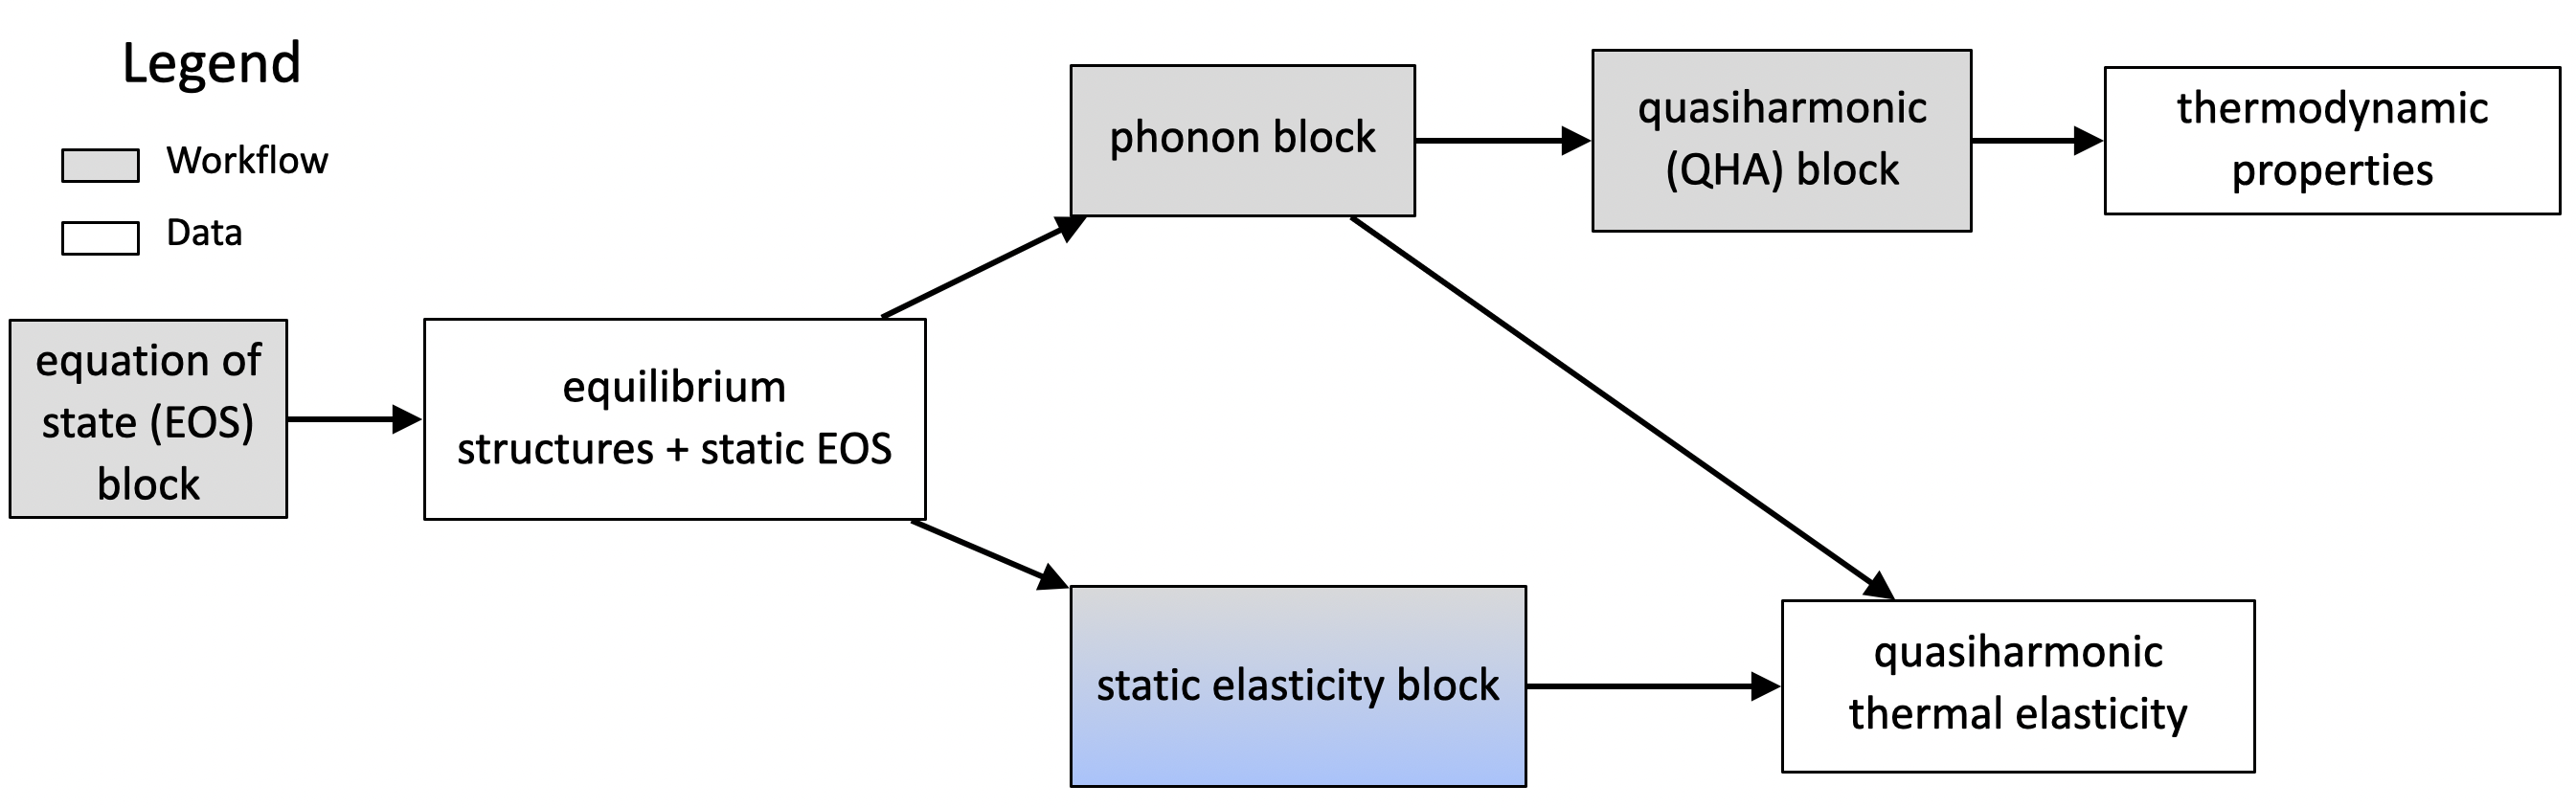
\includegraphics[height=0.4\textheight]{workflows}
        \caption{Typical \ab{} workflows used in our group}
        \label{eq:workflows}
    \end{figure}
\end{frame}

\subsubsection{Binary dependencies and foreign function interface}

\begin{frame}{Build an artifact}

    Operations like finding the symmetry of a crystal,
    are very common in \ab{} calculations (usually the first step).
    Therefore, we need a good library to do this.

    There is a C library called \href{https://github.com/spglib/spglib}{\texttt{spglib}}
    that does this.
    To take this library in productive use, we need first put it in a container
    (``Artifacts''). Luckily, the amazing Julia community has made it possible:
    \href{https://github.com/JuliaBinaryWrappers/spglib_jll.jl}{\texttt{spglib_jll.jl}}.

\end{frame}

\begin{frame}[fragile]{Foreign function interface}

    \begin{columns}
        \begin{column}{0.3\textwidth}
            Now that we have an artifact that exports the functions of the C library,
            it may still be hard to use since it uses some C data structures and API still which may
            not be idiomatic Julia. Therefore, we need to wrap it with a higher level of APIs:
            \href{https://github.com/singularitti/Spglib.jl}{\texttt{Spglib.jl}} is built based on
            this expectation.
        \end{column}

        \begin{column}{0.7\textwidth}
            {\tiny
                \begin{algorithmblock}
                    \begin{juliaverbatim}
function standardize_cell(
    cell::Cell;  # `Cell` was not defined in the C library
    to_primitive = false,
    no_idealize = false,
    symprec = 1e-5,
)
    @unpack lattice, positions, types = _expand_cell(cell)
    to_primitive = Base.cconvert(Cint, to_primitive)
    no_idealize = Base.cconvert(Cint, no_idealize)
    num_atom = Base.cconvert(Cint, length(types))
    allocations = 4
    _positions = Matrix{Cdouble}(undef, 3, num_atom * allocations)
    _types = Vector{Cint}(undef, num_atom * allocations)
    _positions[:, 1:num_atom] = positions
    _types[1:num_atom] = types
    num_atom_std = ccall(
        (:spg_standardize_cell, libsymspg),
        Cint,
        (Ptr{Cdouble}, Ptr{Cdouble}, Ptr{Cint}, Cint, Cint, Cint, Cdouble),
        lattice,
        _positions,
        _types,
        num_atom,
        to_primitive,
        no_idealize,
        symprec,
    )
    if num_atom_std <= 0
        throw(SpglibError("Cell standardization failed!"))
    end
    return Cell(transpose(lattice), _positions[:, 1:num_atom_std], _types[1:num_atom_std])
end
                    \end{juliaverbatim}
                \end{algorithmblock}
            }
        \end{column}
    \end{columns}

\end{frame}

\begin{frame}[allowframebreaks]{Parsers for \ab{} software input and output}

    This is usually hard since most \ab{} are written in Fortran and Julia does not (?)
    have a Fortran parser...

    \framebreak

    \begin{itemize}
        \item For example, \qe{}'s input adopts the \texttt{Namelist} data structure from
              Fortran, and Julia does not have a parser for that...
        \item I know a Python package called
              \href{https://github.com/marshallward/f90nml}{\texttt{f90nml}}, it works well.
              So it came to me that I might write a Julia package that calls that Python
              code.
        \item Therefore, I wrote a very preliminary package
              \href{https://github.com/singularitti/PyFortran90Namelists.jl}{\texttt{PyFortran90Namelists.jl}}
              since writing a parser is time-consuming for a non-CS student like me.
        \item However, it uses \texttt{PyCall.jl}, so sometimes people have trouble installing
              it if they already have Python installed
              (see \href{https://github.com/JuliaPy/PyCall.jl\#specifying-the-python-version}{``Specifying the Python version''}).
    \end{itemize}

    \framebreak

    For output files, it is even more complicated since they usually do not have a standard
    format, therefore lots of regular expressions need to be used.

    It is extremely tricky and error-prone. If you are not familiar with regular expressions,
    try \href{https://github.com/jkrumbiegel/ReadableRegex.jl}{\texttt{ReadableRegex.jl}} to help you build them.

\end{frame}

\begin{frame}[fragile, allowframebreaks]{A wrapper for \ab{} software executables}

    To run external \ab{} software within Julia, what should we do?

    Use the Julia \texttt{AbstractCmd}s? Good choice! But sometimes we want to dynamically generate
    a series of \texttt{AbstractCmd}s. Writing them one by one is not so efficient.

    Or, can we write functions to generate \texttt{AbstractCmd}s? Then all the command
    arguments will be standard Julia function arguments. For example,

    {\scriptsize
            \begin{algorithmblock}
                mpirun -np 16 pw.x -npool 2 -nk 2 -input scf.in > scf.out
            \end{algorithmblock}
        }

    will be

        {\scriptsize
            \begin{algorithmblock}
                \begin{juliaverbatim}
pw("scf.in", "scf.out"; np = 16, npool = 2, nk = 2)
                \end{juliaverbatim}
            \end{algorithmblock}
        }

    \framebreak

    What's more, we could use
    \href{https://github.com/comonicon/Comonicon.jl}{\texttt{Comonicon.jl}},
    to build new executables that will provide customized arguments
    (see \href{https://github.com/MineralsCloud/QuantumESPRESSOCommands.jl}{\texttt{QuantumESPRESSOCommands.jl}})

        {\scriptsize
            \begin{algorithmblock}
                \begin{juliaverbatim}
@cast function pw(input, output = mktemp(parentdir(input))[1]; 
                  np = 1, npool = 1, nk = 1, path = "pw.x", chdir = false)
    ...
    return run(cmd)
end
                \end{juliaverbatim}
            \end{algorithmblock}
        }
        
    Therefore, we could run it with
    {\scriptsize
        \begin{algorithmblock}
            pw -np 16 -npool 2 -nk 2 -input scf.in scf.out
        \end{algorithmblock}
    }

\end{frame}
